\section{Recurrent NNs, Attention \& Transformers}
\subsection{Sequence-to-Sequence Models}
\begin{itemize}
	\item To motivate the later topics in this lecture, one question we should answer
		is how we deal with variable length inputs. In the case of protein folding,
		you have different length sequences for different proteins, so how do you get
		your neural net to predict parameters like the stability, or structure of the
		protein?

		In the most interesting case, your output is contingent on the length of your
		input. This is the case in language translation. 
	\item In general, you need a way to handle variable length inputs, and models
		that do this are called \textbf{sequence-to-sequence models}.
	\item Let's first consider only variable length inputs, so we have something
		like:
		\begin{align*}
			x_1 &= (x_{1, 1}, x_{1, 2}, x_{1, 3}, x_{1, 4})\\
			x_2 &= (x_{2, 1}, x_{2, 2}, x_{2, 3}) \\ 
			x_3 &= (x_{3, 1}, x_{3, 2}, x_{3, 3}, x_{3, 4}, x_{3, 5}) 
		\end{align*}
		because you want to have variable length inputs, you can't just feed the
		neural network the entire \( x_1 \) because then you lose the ability to have
		variable length. 
	\item One possible way you could do this is to feed each dimension of the input
		vector sequentially. That is, for \( x_1 \), we first feed it in \( x_{1, 1}
		\), then \( x_{1, 2} \), then \( x_{1, 3} \), etc. As a diagram:
		\begin{center}
			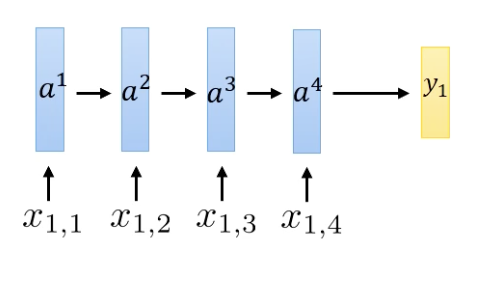
\includegraphics[scale=0.7]{images/lec11-1.png}
		\end{center}
		so, the output \( a^{3} \) hinges on the output \( a^2 \), and so on.
		For inputs with shorter length, we can just prepend a bunch of zeros, which
		does nothing to the data.
	\item In principle, this would work, but the major problem with this direct
		approach is that the number of layers in your network is equal to the length
		of the largest input. If you have very few long inputs, then the model won't
		be very good at predicting the long inputs because there isn't enough data
		out there. 

		To fix this, we tie the layer parameters together, which is called a
		recurrent neural network. It's called recurrent because each \( a^{\ell} \)
		depends recursively on \( a^{\ell - 1} \). 
	\item Something else you could do is to have an output for each input, and
		"decode" the output from that specific layer. The computation is the same,
		the only thing we've changed is that we're decoding the information at every
		step. 
	\item You could also use what's called an \textbf{autoregressive model}, which
		uses the output of the previous iteration to generate the next output. This
		is what ChatGPT does. 

		\question{How is this model different than the first one?} 

		\answer{You are getting the output at every step here, in the first type
			you're not. In other words, you're getting the output of each next word,
		which is generated based on the prevoius word.} 
	\item From this process, hopefully it's clear that there's this general setup
		going on: you have an encoder that "encodes" the input data, and a decoder
		that you run through your neural network to decode the output. That is, the
		general structure could look something like this:
		\begin{center}
			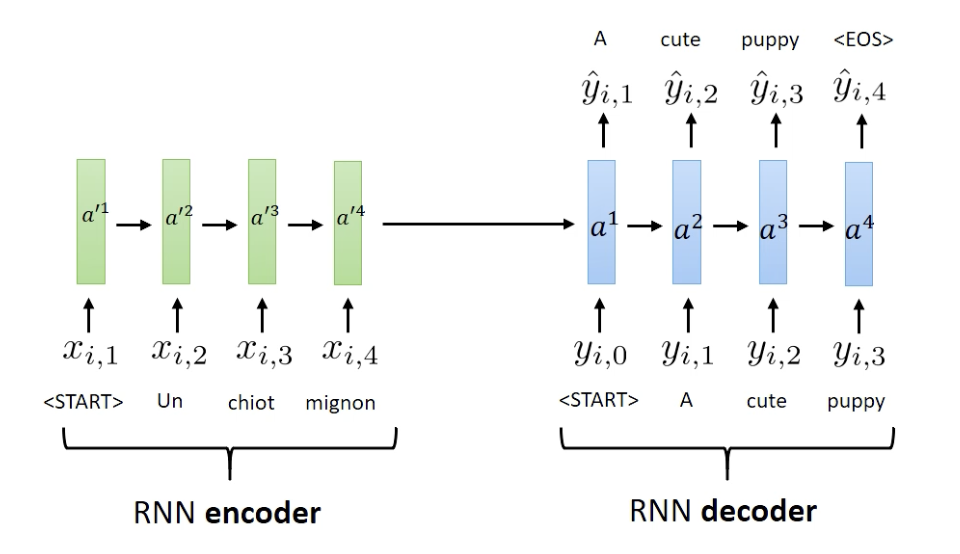
\includegraphics[scale=0.6]{images/lec11-2.png}
		\end{center}
		Note that the RNN encoder could be replaced by a CNN encoder if we were
		dealing with images. Point is, you have a neural network that
		\textit{encodes} the input data, and a decoder that \textit{decodes} the
		data. 

		The encoder translates the input into a "content vector" that describes the
		content, then the RNN decoder does the actual translation.    
\end{itemize}
\subsection{RNN Bottleneck, Attention}
\begin{itemize}
	\item One major problem with this encoder-decoder structure is the transition
		between the encoder and the decoder, called the bottleneck. In essence, if
		you have very long recurrences, then the earlier features that are passed in
		tend to get washed out the longer your recurrence goes. 

		This is the motivation for solutions that involve attention and transformers.
	\item Suppose you don't want all the information to be bottlenecked by the last
		output of the encoder, is there a way we can just translate intermediate
		outputs? The answer is yes, via attention. 
	\item Imagine the standard recurrent neural network (image below), and 
		you're trying to decode \( s_2 \). 
		\begin{center}
			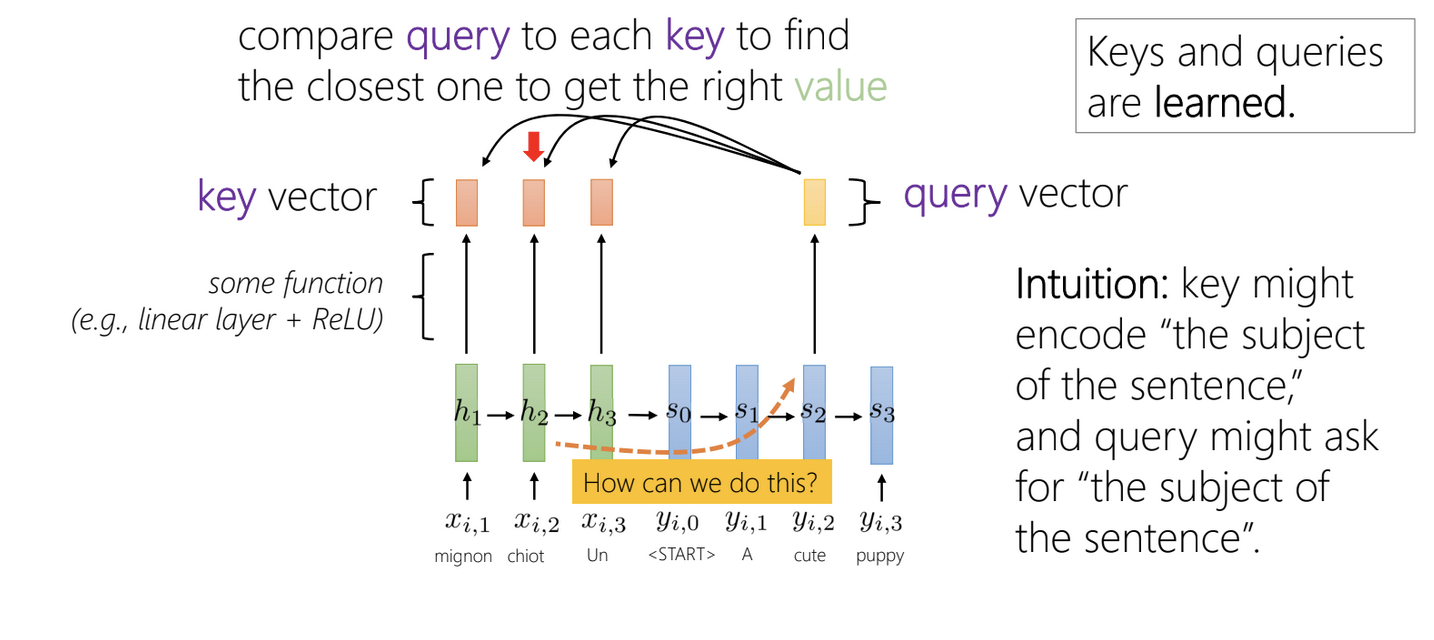
\includegraphics[scale=0.5]{images/lec11-3.png}
		\end{center}
		we can generate a query vector based on the hidden state at \( s_2 \), that
		allows us to query back in time and look for matches. This is a probabilistic
		lookup, so it picks the one that has the highest similarity, based on some
		heuristic (maybe a dot product or something).     

		\comment{The intuition to have is that if you're trying to decode the subject
			of the sentence, the query vector goes back in time and looks for the
		subject of the sentence from the encoder.}
	\item Refer to the diagram below:
		\begin{center}
			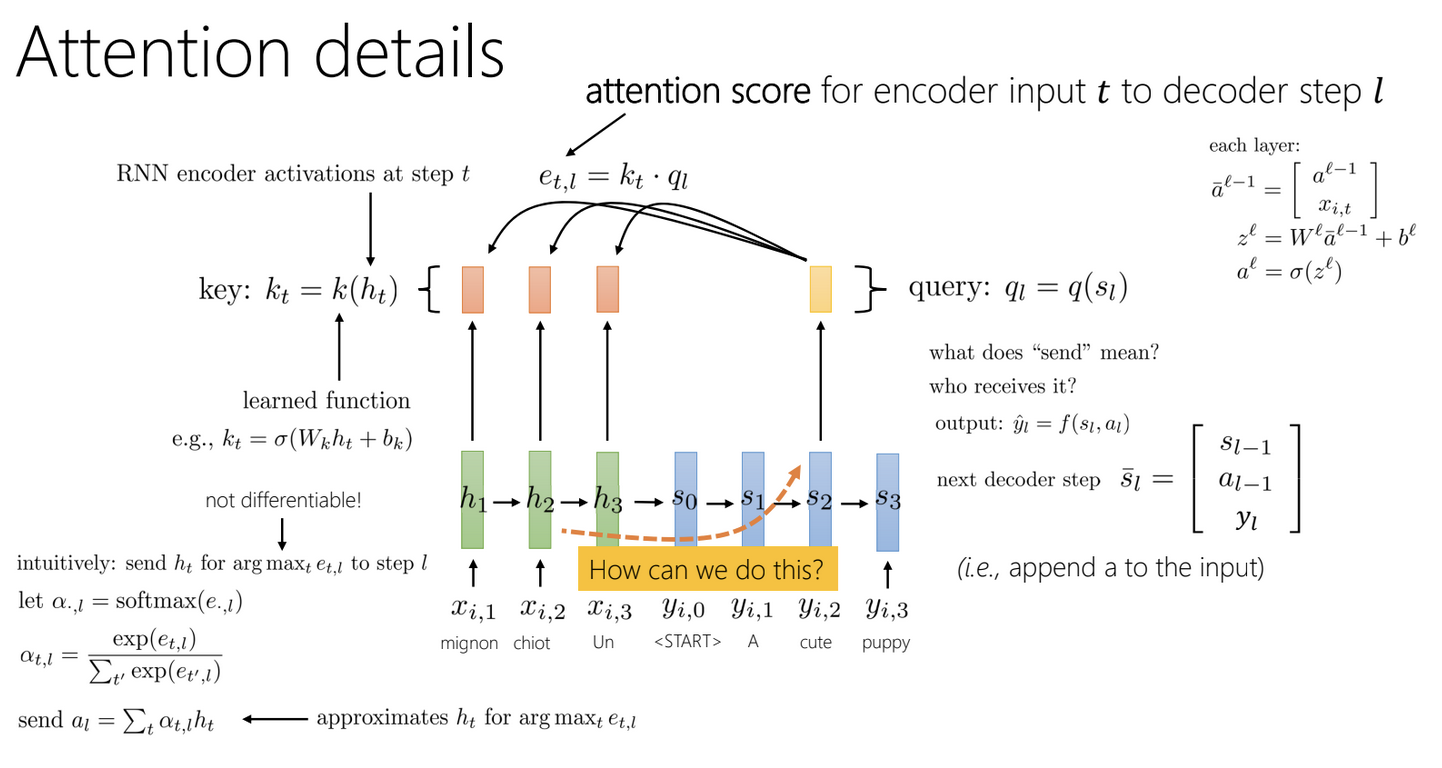
\includegraphics[scale=0.5]{images/lec11-4.png}
		\end{center}
		\begin{itemize}
			\item Suppose you're at \( s_2 \), and you're looking to query.
				To compute the keys, you take the hidden input \( h_t \) at 
				every layer, and you put it through a function \( k(h_t) \). \( k \) 
				could be as simple as the identity, but it can also be a simple 
				learned function as well (e.g. \( k_t = \sigma(W_k h_t + b_k) \)). 
			\item When you're query, you put it through a query function \( q_{l} =
				q(s_l) \). \( q_l \) is a vector representing some concept, and
				we take the inner product of \( q_l \) with every input \( k_t \).
				This quantity \( e_{t, l} \) is called the \textbf{attention score}.  
			\item Intuitively, we would like this to be a database lookup, which
				would basically be the same as looking for \( \argmax e_{t, l} \).
				But, because this is not differentiable, we normally use a softmax
				instead.  That is:
				\[
					\alpha_{t, l} = \frac{\exp(e_{t, l})}{\sum_{t'} \exp(e_{t', l})}
				\]
				Now, the combination of all of these is a normalized probability
				distribution, then we take a linear combination of the attention
				score with the information in the input sequence back. That is, we
				send \( a_l = \sum_t \alpha_{t, l} h_t \) back. Basically, this
				ensures that the things which are sent back with high probability are
				the ones that correspond highly with the data.  
			\item After sending \( a_l \) back, we can then use this information
				combined with \( s_2 \) to finally get a prediction \( \hat{y}_{2}
				\).   
			\item The number of attention scores you have depends on the length of
				the input string. The computational complexity is then dependent on
				the length of your input. 
		\end{itemize}
	\item Some general examples of \( k(t) \) and \( q(t) \) are just the identity
		function:
		\[
			k_t = h_t \quad q_l = s_l
		\]
		so the decoder is just the inner product between the encoder and decoder. You
		can also use more complicated functions, such as:
		\[
			k_t = W_k h_t \quad q_l = W_q s_l
		\]
		where \( W \) is a parameter we augment by (\question{is this learned?}). On
		the decoder side, you then have:
		\[
			e_{t, l} = h_{t}^{\top} W_k^{\top} W_q s_l = h_{t}^{\top}W_e s_l
		\]
	\item You can also do weird things with the returned \( a_l \) as well. Instead
		of just taking the dot product of the attention score with each layer, you
		can also use a learned function here, so you return
		\[
			a_l = \sum_t \alpha_t v(h_t)
		\]
		where \( v(h_t) \) is some learned function.  

		\question{We keep saying this "learned function", how do you learn functions
		like this? Do you have another neural net that does this?}
	\item Attention is a \textbf{very} powerful tool! There is no longer a bottleneck
		because each layer can just use attention. This is very similar to how
		resents work -- we're shortening the gradient path, so this makes the neural
		net better. 
\end{itemize}
\subsection{Transformers}
\begin{itemize}
	\item Is attention all we need? Do we even need the recurrence or the
		autoregressive model? The answer is no, and what we can actually do is just
		rely only on attention. This is what transformers are. 
	\item The only issue you have with the current model is that you can only look at
		the key vectors for the input pairs, but not the decoding layers. To solve
		this, we implement \textbf{self-attention}. So, we basically make a key
		vector for \textit{every layer}, including the ones in the decoding network.
	\item Refer to the following diagram:
		\begin{center}
			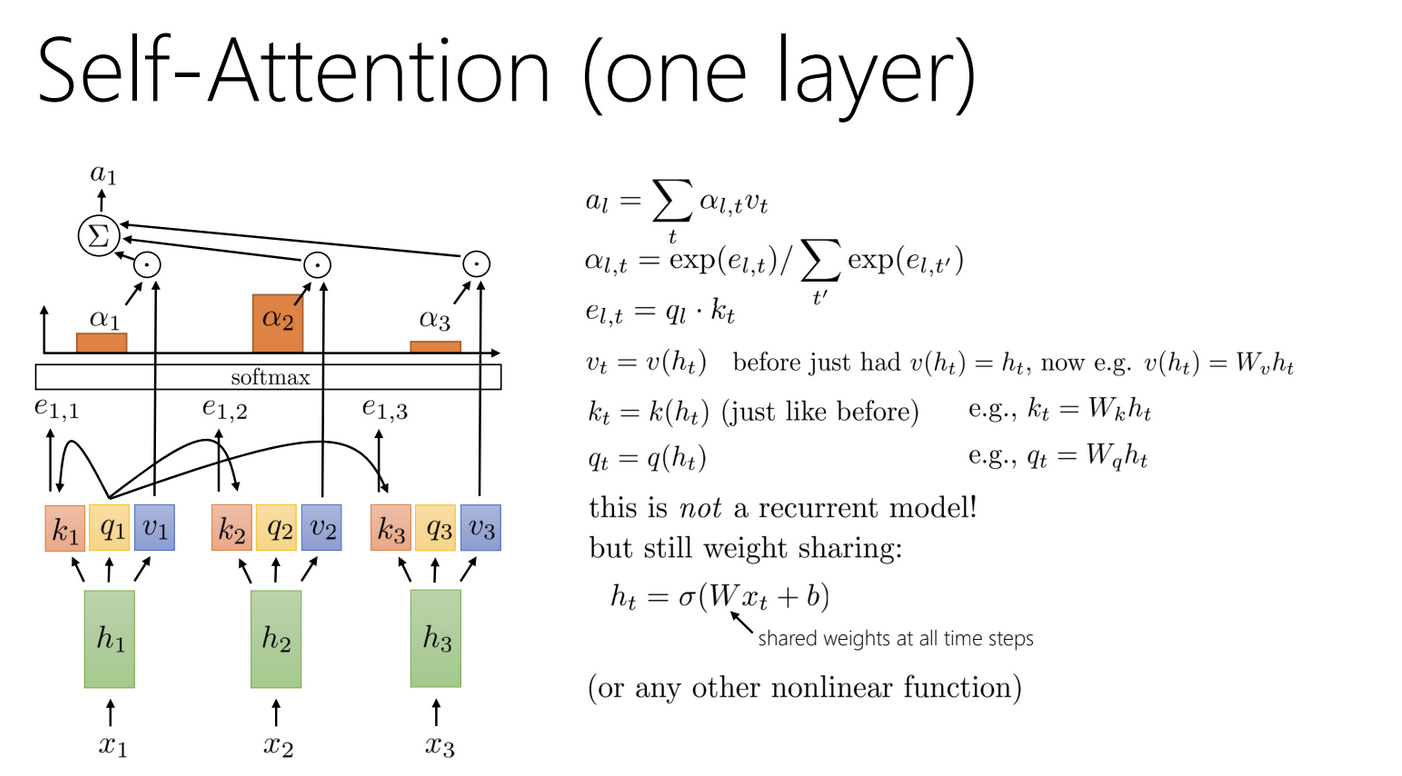
\includegraphics[scale=0.5]{images/lec11-5.png}
		\end{center}
		\begin{itemize}
			\item The intermediate arrows are now gone, and instead it's replaced by
				these \( k_i, q_i, v_i \) values. We still have a shared weight \(
				h_t = \sigma(W x_t + b) \), but they are no longer connected to each
				other. 
			\item Now, each layer has a value \( v_t \), which is defined by \(
				v(h_t) \), just as before. The key vector is also stored, in the same
				way as before \( k_t = k(h_t) \). The query is also the same as
				before. 
			\item So basically, this is a very dense version of what we had before --
				instead of having the keys in the encoder and the queries in the
				decoder, they are now all in the same system (so to speak). 
			\item If you're querying for \( h_1 \), then you query through \( k_1,
				k_2, k_3 \), and compute the attention in the same way we did before.
				The only difference is that you're querying your own key \( k_1 \) as
				well. 
			\item \( a_l \) is defined the same way, through the softmax, etc. 
		\end{itemize}
	\item Now that we've removed the recurrence, this means that the network is now
		permutation equivariant: if you switch up the order of \( h_i \) the output
		doesn't change, which is bad.  
	\item You can also stack attention layers on top of each other in the same way
		you stack a convolutional neural network. 
	\item Some issues with our model so far:
		\begin{itemize}
			\item Lack of sequence information: by removing the recurrence we've
				removed the ordering.  

				To fix this, we just force-feed position information into \( h(t) =
				f(x_t, t)\). If you just feed it in something simple (like 1, 2, 3,
				...), it actually
				doesn't do very well. What people actually do is give it a positional
				encoding \( p_t \) which is a giant vector of sines and cosines. 
			\item Multi-headed attention: in the same way you can have multiple
				kernels for your neural network, you can also have an attention layer
				for each kernel, which is called multi-headed attention.
				
				You can do multi-headed attention in parallel, the mechanisms are
				exactly the same, except in a higher dimension because we have more
				queries, keys, and values. 
			\item Linearity: each successive layer is linear in the previous one

				Fixing this just requires you to add a some nonlinear function in
				between the attention layers. 
			\item Masked decoding: How do we prevent attention lookups into the
				future?  

				This is mainly an issue caused by addressing the first issue -- when
				we bake an ordering into the system, then we have to restrict what
				each layer can query, which we can do by modifying the dot product to
				be:
				\[
					e_{l, t} = \begin{cases}
						q_l \cdot k_t & t \leq l\\
						-\infty & \text{otherwise}
					\end{cases}
				\]
				This solves the issue because now you'll get a \( -\infty \)
				attention score for the things you're not supposed to look at. 
				
				\comment{Note that throwing this into the softmax will give you \(
				e^{-\infty} = 0 \), so it does work out as expected.}
		\end{itemize}
	\item And now we've essentially built a transformer. Nowadays, transformers
		usually just refer to this stacking of self attention layers. 
	\item Some downsides is that this is pretty slow, as it runs in \( O(n^2) \),
		compared to \( O(n) \) (roughly) due to backpropagation. It's also slightly
		harder to implement. 

		That said, it also has many benefits, which outweigh the downsides: they have
		much better long-range connections, they're much easier to parallelise, and
		you can also make them much deeper than you can with RNNs.  
\end{itemize}
